\chapter{Design}
\label{design}
\section{Program Requirements}
\label{programRequirements}

\subsection{Motivation}
While the detriments to SAON technologies are well-known \cite{Akbarzadeh2013}, \cite{Heupel2006}, \cite{Howard2002},  \cite{Kessel2015}, \cite{Steel2014} there few tools/services to analytically design SAONs around them.  Further, none of these tools/services are free and open-source.


\subsubsection{Cost Efficiency}
\label{motivationCost}
In section~\ref{CostAltTech}, we discuss the costs of marine telemetry systems, noting that acoustic telemetry systems produce data at a significantly lower ($\ge$10x cheaper) cost than VHF or GPS/Satellite based technologies.  In order to maintain the cost-efficiency of acoustic technology, at least 10$\%$ of the produced transmissions must be captured by the SAON's receiver array.  Given the numerous (but avoidable) impediments to reception of these acoustic signals (\ref{RulesOfThumb}), the array-design process becomes critical to maintaining the cost-efficiency of SAON technologies.  A free network design tool would help to maintain the cost-efficiency of SAONs by eliminating costs surrounding their design and evaluation.  


\subsubsection{Metrics}
\label{motivationMetrics}
The computation of network metrics (Absoloute Recovery Rate, Unique Recovery Rate, Network Sparsity) is very labor intensive at large scale.  Additionally, the process of computation may vary from experiment to experiment.  An automated tool would solve both issues by providing a fast, simple, repeatable, and well-documented method for computation.  Metrics from such a tool would be useful in directly comparing different network deigns.


\subsubsection{Transparency}
\label{motivationTransparency}
An open-sourced tool/service would make the design process more transparent, permitting peer-review and modification.  This would provide increased confidence in the process, and increased adoption of the tool.  Increased adoption would result in a larger number of efficient SAONs, leading to higher data recovery rates, better data quality, increased return-on-investment, and the ability to better address scientific-research questions.


\subsection{Supported Workflows}
\label{workflows}
\subsubsection{Static Analysis}
\label{staticAnalysis}
As mentioned in section~\ref{motivationMetrics}, a primary motive for this tool was the ability to create a repeatable means of measuring the performance of a SAON.  To this end, the ability to measure an existing network design is important.  Users should be presented with network metrics after specifying bathymetry, receiver locations, network properties, and an animal model for a given study site.


\subsubsection{Optimal Design}
\label{optimalDesign}
The primary motive for this tool is the ability to design optimal SAONs.  Users should be presented with a network design (optimal receiver locations), and network metrics after specifying bathymetry, the number of receivers in the network, network properties, and an animal model for a given study site.


\subsubsection{Optimal Addition}
\label{optimalAddition}
Similar to the problem of optimal design, is the problem of optimal addition: the augmentation of an already existing SAON.  Users should be presented with a network design (optimal augmenting receiver locations), and network metrics after specifying bathymetry, the number of receivers to add to the network, network properties, existing receiver locations, and an animal model for a given study site.

\section{Conceptual Model}
\label{conceptualModel}
\subsection{Time/Space Modeling}
\label{timeSpaceModel}
\subsubsection{Spatial Modeling}
\label{spatialModeling}
To model a 3-dimensional underwater environment, we start with a two-dimensional grid of cells (in the x and y dimensions) containing numerical values.  Numerical values in those cells can then be used in static shape functions to generate the third dimension (z) for that cell.  In this way, we save significant amounts of memory by compute values for a specific three-dimensional cell on the fly, instead of storing an additional dimension.  

\subsubsection{Temporal Modeling}
\label{temporalModeling}
With respect to the passage of time, our model assumes that receivers are stationary throughout the entire experiment.  Furthermore, the animal model does not represent animal movement over time, but the percentage of time an animal would spend in a particular cell over the entire study period.  The animal model therefore represents the tendency of an animal's movements over the expected study period rather than its particular movements in a small time period.  As a result, we need not consider temporally-related phenomena. 

Bathymetry files are generally given as grids of depths, with varying cell sizes.  The resolution of a bathymetric file is given by the dimensions of its cells.  For example, a 50 meter Bathymetry file has cell sizes of approximately 50 meters square (although these cells are not necessarily perfectly square).  Bathymetric files list beginning and ending coordinates (North/South Latitudes and East/West Longitudes), as well as the grid size (in rows and columns) in cells.  With these two measurements, one can compute the degrees per cell of latitude and longitude.  Thus, particular latitudes and longitudes can be converted to rows/columns, and back.  


\subsection{Bathymetric Modeling}
\label{bathymetyricModeling}
\subsubsection{Bathymetric Grid}
\label{bathymetricGrid}
Our program works on a grid-based system, taking advantage of the grid system given by the bathymetric file.  Thus, the resolution of our program's output is dictated by the resolution of the input bathymetric file.  While it may seem useful to have the ability to artificially increase the resolution of the simulation by sub-dividing the input cells into sub-cells of smaller resolution, doing so increases the computational size of the program without meaningfully increasing the resolution of the results.  The primary component of the program is the bathymetric file.  Both the animal model and the bathymetric shadowing model make decisions based upon the depth at a particular cell.  
//TODO: discuss filetype support


\subsubsection{Bathymetric Resolution}
\begin{figure}
	\label{resolutionScale}
	\begin{subfigure}[t]{.4\textwidth}
		\centering
		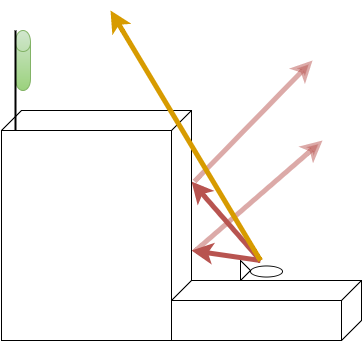
\includegraphics[width=\linewidth]{LoS.png}
		\caption{}\label{LoS}
	\end{subfigure}
	\begin{subfigure}[t]{.4\textwidth}
		\centering
		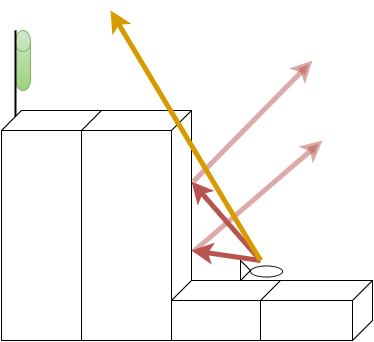
\includegraphics[width=\linewidth]{duplicate.png}
		\caption{}\label{duplicate}
		
	\end{subfigure}
	
	\begin{subfigure}[t]{.4\textwidth}
		\centering
		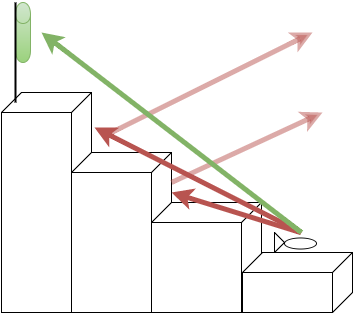
\includegraphics[width=\linewidth]{smooth.png}
		\caption{}\label{smooth}
	\end{subfigure}
	\caption{Figure~\ref{LoS} illustrates the bathymetric shadowing model on a bathymetric grid.  Figure~\ref{duplicate} shows how artifically increasing the resolution of the bathymetric grid form Figure~\ref{LoS} using the duplication method of cell sub-division does not affect the bathymetric shadowing model.  Figure~\ref{smooth} shows how artificially increasing the resolution using a smoothing function can lead to inflated signal reception.}
\end{figure}
When subdividing cells, either the sub-cells are given the same depth as their parent cell, or the depth of a sub-cell is interpolated from surrounding cells by some smoothing function.  Subdividing a cell into sub-cells with the same depth makes the assumption that all sub-cells are actually the same depth.  Furthermore, this results in the animal and bathymetric shadowing models making the same depth-based decision for all sub-cells that they would for the larger parent cell, increasing the computational load (see Figure~\ref{duplicate}).  Subdividing a cell into sub-cells with a depth governed by a smoothing function makes the assumption that there are no impeding obstacles between neighboring cells, and that there is a smooth transition between them (see figure~\ref{smooth}).  Both strategies for artificially increasing the resolution of a bathymetric file disregard the manner in which the bathymetry was originally observed.  Bathymetry is almost always computed as an average depth for an area of a given size (resolution).  For example, imagine a cell with a steep cliff running across the middle.  This cell would have a depth equal to the average of the depth at the top of the cliff and the base of the cliff.  This average is the depth that would be recorded in the bathymetric file.  Subdividing this cell into four sub-cells of the same depth would indicate to the acoustic model that acoustic signals can pass freely across this cell.  In reality, acoustic signals would be severely hampered by the cliff face.  Subdividing this cell into four sub-cells with depths given by a smoothing function would result in the large depth change at the sheer cliff face being smoothed into smaller changes in depth, which would allow significantly better transmission of acoustic signals than a single large cliff face.

 
\subsection{Bathymetric Shadowing}
\label{bathymetricShadowing}
In reality, the transmission of an acoustic ping originates from the tagged animal and propagates to the receiver.  This propagation is governed by complex interactions with the surrounding environment (including the bottom substrate, distance to the surface/sea-floor, thermoclines, the number of tagged animals in the vicinity, and ambient noise).  Because it is difficult to model these phenomena without significant data on a large number of variables over a large area, we utilize a simplified propagation model relying on direct line of sight between a tagged animal and a receiver.  Simply put, in order to receive a transmission, there must exist a topographically-unobstructed path between a tagged animal and a receiver.  A naive solution might be to determine whether or not each cell in the three-dimensional grid can see the receiver.  Recall however, that we are using a 2-dimensional grid as the basis of our simulation and computing the third dimension as necessary.  Therefore, it is much more computationally efficient to determine the deepest depth in each cell that can be seen by the receiver.

\subsection{Evaluation of Sensor Emplacements}



\subsection{Selection of Optimal Emplacements}




\section{Animal Modeling}
Animals exhibit many different movement models and habitat preferences (both of which can vary in three-dimensional space).  This greatly affects their distribution and thus the network configuration that should be deployed to capture their movement.  Our program models account for both the habitat and movement preferences of the target species by allowing for various optional parameters and functions.

\subsection{Animal Movement Models}
 To simulate tagged animal movement across a two dimensional x/y space (as one would expect to see on a map), we provide two basic probabilistic movement models: Random Walk, and Ornstein-Uhlenbeck(OU).  

\paragraph{Random Walk Model}
The Random Walk model assumes that animals move randomly through the environment.  As a result, over the entire study period, each valid grid cell (as defined by vertical habitat range) will see an equal amount of animal traffic.  The result is that every valid cell  in the grid will have the same chance of capturing an animal's acoustic transmission.  We assume that tagged individuals will be willing and able to very briefly (in probabilistically negligible time frames) pass through inhospitable (over dry land, through impassible terrain) cells to get to other cells.  This means that disjoint sections of habitat are still equally likely to see animal movement/presence.

\paragraph{Ornstein-Uhlenbeck Model}
The Ornstein-Uhlenbeck(OU) model\cite{OU} assumes that over time, animals will prefer to gather near certain points of interest.  This concept models an animal's desire to seek out and remain near a physically significant structure, a region of high food availability, breeding grounds, shelter, etc.  Users must provide the x and y coordinates for this point (as grid indicies), the strength of attraction in the separate x and y directions, and the correlation between the x and y attraction as parameters to the program.  


\subsection{Simulated Animal Depth Preference}
Some animals exhibit the preference to reside within a specific section of the water column; for example, prey animals may prefer hiding in reef heads at the bottom of the water column, while predators will prefer to hover several meters off the bottom.  This preference can be incorporated into the behavioral model by specifying mean (Preferred Depth) and standard deviation(SD of Preferred Depth) values.  These values are given as a measure of the distance (in meters) from the bottom.  For example, specifying a depth of '0' for "Preferred Depth" indicates that the animal prefers to live on the sea floor, while a value of '5' indicates that the animal prefers to live 5m off the sea floor.  Allowing a standard deviation value allows for the modeling of animals that tend to be sedentary within the water column (a small deviation), and those that migrate through the water column (a large deviation).

\subsection{Restricted Vertical Habitat Range}
Some animals will live only in a specific depth range.  For example, a deep sea fish may live only in depths of 300-400 meters.  To incorporate this into the behavioral model, users can specify a minimum and maximum vertical habitat range for their animal.  If this option is selected, the program will only simulate animals in cells whose depths are between the minimum and maximum depths.  As in the Random Walk Model, we assume that animals are willing and able to move between disjoint areas of habitat.


\section{Sensor Projection}
In normal research situations, users will have a set number of sensors to place within their study site.  The process of arriving at this number is likely unscientific, perhaps relying on user estimate (such as the user-perceived feasibility of receiving a given number of receivers).  Rather than guessing at the number of sensors to use, and hoping for an adequate data recovery rate, users should be able to calculate the marginal benefit (additional detections, increased Data Recovery Rates) of utilizing a variable number of receivers.   To this end, the program allows for the projected incremental benefit for a given number of additional receivers.  Our program facilitates this by allowing users to specify a number of sensors to project, returning graphs and metrics of the marginal increase in Data Recovery Rate.  Armed with this data, users can determine an appropriate number of receivers to purchase, or construct an argument for purchasing more receivers.

\section{Network Model Ingestion}
\subsection{Customizable Network Models}
The program supports three distinct ways to define sensors in a network: 
user specific ation, program-placed sensors, and projected sensors. 
User placed sensors represent sensors that already exist, and are being integrated into a new network.
Program placed sensors are sensors that are optimally placed by the program, and take into account any user placed sensors.
Projected sensors are 
Add new sensors (with optimal placement) to an already existing network
Analyze the data recovery rate for a sensor network
Create an optimal sensor network

\section{Goodness Algorithms}
\subsection{Selectable Goodness Algorithms (Bias)}
The “Goodness” algorithm is the driving force behind the selection of sensor placements.  While users are able to write their own “Goodness” algorithms, three basic algorithms are provided: 

\paragraph{Animal Only (Option “1”)}
This option prefers to place sensors in areas of high animal activity, completely oblivious to the surrounding topography.  

\paragraph{Topography Only (Option “2”)}
This option places sensors in areas that have the best visibility of the surrounding area.  This is useful for experiments where animal habitat is unknown or to be determined.

\paragraph{Visible Fish (Option “3”)}
This option chooses sensor locations that have the best view of areas of high animal activity.  Both animal presence and visibility due to topography are considered.
